% Template for Elsevier CRC journal article
% version 1.2 dated 09 May 2011

% This file (c) 2009-2011 Elsevier Ltd.  Modifications may be freely made,
% provided the edited file is saved under a different name

% This file contains modifications for Procedia Computer Science

% Changes since version 1.1
% - added "procedia" option compliant with ecrc.sty version 1.2a
%   (makes the layout approximately the same as the Word CRC template)
% - added example for generating copyright line in abstract

%-----------------------------------------------------------------------------------

%% This template uses the elsarticle.cls document class and the extension package ecrc.sty
%% For full documentation on usage of elsarticle.cls, consult the documentation "elsdoc.pdf"
%% Further resources available at http://www.elsevier.com/latex

%-----------------------------------------------------------------------------------

%%%%%%%%%%%%%%%%%%%%%%%%%%%%%%%%%%%%%%%%%%%%%%%%%%%%%%%%%%%%%%
%%%%%%%%%%%%%%%%%%%%%%%%%%%%%%%%%%%%%%%%%%%%%%%%%%%%%%%%%%%%%%
%%                                                          %%
%% Important note on usage                                  %%
%% -----------------------                                  %%
%% This file should normally be compiled with PDFLaTeX      %%
%% Using standard LaTeX should work but may produce clashes %%
%%                                                          %%
%%%%%%%%%%%%%%%%%%%%%%%%%%%%%%%%%%%%%%%%%%%%%%%%%%%%%%%%%%%%%%
%%%%%%%%%%%%%%%%%%%%%%%%%%%%%%%%%%%%%%%%%%%%%%%%%%%%%%%%%%%%%%

%% The '3p' and 'times' class options of elsarticle are used for Elsevier CRC
%% The 'procedia' option causes ecrc to approximate to the Word template
\documentclass[3p,times,procedia]{elsarticle}
\flushbottom

%% The `ecrc' package must be called to make the CRC functionality available
\usepackage{ecrc}
\usepackage[bookmarks=false]{hyperref}
    \hypersetup{colorlinks,
      linkcolor=blue,
      citecolor=blue,
      urlcolor=blue}
%\usepackage{amsmath}


%% The ecrc package defines commands needed for running heads and logos.
%% For running heads, you can set the journal name, the volume, the starting page and the authors

%% set the volume if you know. Otherwise `00'
\volume{00}

%% set the starting page if not 1
\firstpage{1}

%% Give the name of the journal
\journalname{Procedia Computer Science}

%% Give the author list to appear in the running head
%% Example \runauth{C.V. Radhakrishnan et al.}
\runauth{Brozeit et al.}

%% The choice of journal logo is determined by the \jid and \jnltitlelogo commands.
%% A user-supplied logo with the name <\jid>logo.pdf will be inserted if present.
%% e.g. if \jid{yspmi} the system will look for a file yspmilogo.pdf
%% Otherwise the content of \jnltitlelogo will be set between horizontal lines as a default logo

%% Give the abbreviation of the Journal.
\jid{procs}

%% Give a short journal name for the dummy logo (if needed)
%\jnltitlelogo{Computer Science}

%% Hereafter the template follows `elsarticle'.
%% For more details see the existing template files elsarticle-template-harv.tex and elsarticle-template-num.tex.

%% Elsevier CRC generally uses a numbered reference style
%% For this, the conventions of elsarticle-template-num.tex should be followed (included below)
%% If using BibTeX, use the style file elsarticle-num.bst

%% End of ecrc-specific commands
%%%%%%%%%%%%%%%%%%%%%%%%%%%%%%%%%%%%%%%%%%%%%%%%%%%%%%%%%%%%%%%%%%%%%%%%%%

%% The amssymb package provides various useful mathematical symbols

\usepackage{amssymb}
%% The amsthm package provides extended theorem environments
%% \usepackage{amsthm}

%% The lineno packages adds line numbers. Start line numbering with
%% \begin{linenumbers}, end it with \end{linenumbers}. Or switch it on
%% for the whole article with \linenumbers after \end{frontmatter}.
%% \usepackage{lineno}

%% natbib.sty is loaded by default. However, natbib options can be
%% provided with \biboptions{...} command. Following options are
%% valid:

%%   round  -  round parentheses are used (default)
%%   square -  square brackets are used   [option]
%%   curly  -  curly braces are used      {option}
%%   angle  -  angle brackets are used    <option>
%%   semicolon  -  multiple citations separated by semi-colon
%%   colon  - same as semicolon, an earlier confusion
%%   comma  -  separated by comma
%%   numbers-  selects numerical citations
%%   super  -  numerical citations as superscripts
%%   sort   -  sorts multiple citations according to order in ref. list
%%   sort&compress   -  like sort, but also compresses numerical citations
%%   compress - compresses without sorting
%%
%% \biboptions{authoryear}

% \biboptions{}

% if you have landscape tables
\usepackage[figuresright]{rotating}
%\usepackage{harvard}
% put your own definitions here:x
%   \newcommand{\cZ}{\cal{Z}}
%   \newtheorem{def}{Definition}[section]
%   ...

% add words to TeX's hyphenation exception list
%\hyphenation{author another created financial paper re-commend-ed Post-Script}

% declarations for front matter


\begin{document}
\begin{frontmatter}

%% Title, authors and addresses

%% use the tnoteref command within \title for footnotes;
%% use the tnotetext command for the associated footnote;
%% use the fnref command within \author or \address for footnotes;
%% use the fntext command for the associated footnote;
%% use the corref command within \author for corresponding author footnotes;
%% use the cortext command for the associated footnote;
%% use the ead command for the email address,
%% and the form \ead[url] for the home page:
%%
%% \title{Title\tnoteref{label1}}
%% \tnotetext[label1]{}
%% \author{Name\corref{cor1}\fnref{label2}}
%% \ead{email address}
%% \ead[url]{home page}
%% \fntext[label2]{}
%% \cortext[cor1]{}
%% \address{Address\fnref{label3}}
%% \fntext[label3]{}

\dochead{7th International Conference on Industry of the Future and Smart Manufacturing}%%%
%% Use \dochead if there is an article header, e.g. \dochead{Short communication}
%% \dochead can also be used to include a conference title, if directed by the editors
%% e.g. \dochead{17th International Conference on Dynamical Processes in Excited States of Solids}

\title{A Collection-based Digital Product Passport Suitable for Tracking Parts With No ID}

%% use optional labels to link authors explicitly to addresses:
%% \author[label1,label2]{<author name>}
%% \address[label1]{<address>}
%% \address[label2]{<address>}



\author[a]{Jonas Brozeit}
\author[a]{Abdullah Farrukh}
\author[a]{Peter Stein\corref{cor1}}
\author[a]{Christiane Plociennik}
\author[a]{Martin Ruskowski}
%\author[b]{System 180}

\address[a]{German Research Center for Artificial Intelligence (DFKI), Trippstadter Str. 122, 67663 Kaiserslautern, Germany}
% \address[b]{System 180 GmbH, Ernst-Augustin-Straße 3, 12489 Berlin, Germany}

\begin{abstract}
Digital Product Passports (DPPs) are great for collecting, tracking, and using product-related information across different stakeholders along the entire product lifecycle. Usually, a product is linked to its virtual counterpart (the DPP) by a machine-readable identifier (ID) such as a QR code. An open question is how to seamlessly track products or parts of products that carry no ID on them. In this paper, we introduce a DPP concept based on the well-understood concept of a Collection. This approach assumes that each part belongs to a Collection at all times, which makes it trackable without an ID. An object can be removed from a Collection or added to another Collection. We explain our concept via a use case from the System 180 Green-AI Hub pilot project.
We validate the approach with an edge demonstrator and a web application, where computer vision detects components and condition and results are stored in a Neo4j graph. Collections ensure traceability without physical IDs. The experiments demonstrate feasibility, and we discuss limitations and industrial relevance.
\end{abstract}

\begin{keyword}
%% keywords here, in the form: keyword \sep keyword
Collection \sep Digital Product Passport \sep Circular Economy \sep Artificial Intelligence \sep Sustainability-oriented production \\


% more keywords: Digital Twins, Simulation, VR/AR Applications 

%% PACS codes here, in the form: \PACS code \sep code

%% MSC codes here, in the form: \MSC code \sep code
%% or \MSC[2008] code \sep code (2000 is the default)

\end{keyword}
\cortext[cor1]{Corresponding author.}
\end{frontmatter}

%\correspondingauthor[*]{Corresponding author. Tel.: +0-000-000-0000 ; fax: +0-000-000-0000.}
\email{peter.stein@dfki.de}

%%
%% Start line numbering here if you want
%%
% \linenumbers

%% main text

%\enlargethispage{-7mm}


\section{Introduction}
\label{sec:intro}

The upcoming \emph{Ecodesign for Sustainable Products Regulation} (ESPR, COM/2022/142) \cite{ESPRRegulation2022} will oblige many products, including furniture, to carry a \emph{Digital Product Passport} (DPP).  Manufacturers must therefore record each component’s composition, usage history, and end-of-life route.  Achieving that level of traceability in highly modular furniture is still an open challenge.

Modularized and extensible furniture systems are made up of smaller assemblies or singular parts with interconnections, which decrease the effort of reconfiguration and expansion while reducing manufacturing complexity. System 180 offers such a modular and extensible furniture system with various components which can be interconnected to fulfill a purpose, e.g. a shelf for an office or a workbench in a workshop. Besides using new parts to assemble a customer's furniture, the reuse of parts from furniture at the end of its lifecycle is a viable alternative. 

However, this requires careful examination and inventory of decommissioned furniture and its components. Due to the high variety of components, a manual process is not suitable for this task. The automation of the inventory taking task poses major challenges. To assess a component's lifecycle, it must be tracked across different lifecycle stages. Using unique identifiers, such as QR codes or barcodes, is not feasible due to the large number of parts or lack of sufficient placement area on components.

Hence, this paper explores the use of state-of-the-art artificial intelligence (AI) methods, such as object detection and tracking, in combination with semantic technologies like the Asset Administration Shell (AAS), to automate the identification and classification of furniture components using image and video data.

To address the lack of physical identifiers, we apply the \textit{Collection Principle}, which structures digital product representations around dynamic groupings of parts. A collection may represent a physical product (e.g., a workbench), a stockpile, or an individual subassembly. Because each part always belongs to exactly one collection, the system ensures traceability without the need for permanent IDs. Collections can be interactively modified via a user interface, allowing users to transfer subsets into new or existing collections -- supporting processes such as inventory audits, reassembly, or reuse planning.

Additionally, we store all detected relationships and metadata in a Neo4j knowledge graph. This enables advanced queries and inference, including reasoning over components that are not directly visible in an image but may be inferred based on their likely inclusion within a known configuration or context.

We assess the concept using two complementary demonstrators: (1) a web-based application that allows users to upload or capture component images, and (2) a physical demonstrator using embedded hardware and cameras to capture and classify components on-site. With this work, we aim to contribute to key goals of the circular economy and Industry 4.0 by making modular furniture more reusable, identifiable, and semantically linked across its lifecycle.

While prior work has shown effective object detection for assemblies, it rarely connects vision output to a dynamic, lifecycle-spanning representation that enables ID-free tracking. This paper contributes: (1) a Collection-based DPP model that guarantees traceability without physical IDs; (2) an implementation that fuses computer vision with a graph backend for modular furniture; and (3) two demonstrators (edge and web) that validate feasibility in realistic settings.

Section~\ref{sec:related} reviews related work.
Section~\ref{sec:method} outlines the methodology, including concept, model training, information extraction, and DPP integration.
Section~\ref{sec:results} presents results for the physical and web demonstrators.
Section~\ref{sec:discussion} discusses implications and limitations.
Section~\ref{sec:conclusion} concludes with outlook and industrial relevance.

\section{Related Work}
\label{sec:related}

Training AI models to detect and track components of modular furniture requires suitable datasets. Besides real-world data -- typically annotated manually by domain experts using labeling tools such as Label Studio~\cite{Labelstudio} or Roboflow~\cite{dwyer2024roboflow} -- synthetic data can be used to augment or bootstrap model training. Simulation platforms such as Isaac-Sim~\cite{Isaac-Sim} can generate diverse and precisely annotated RGB images, offering scalable training input for object detection models.

Recent literature has demonstrated the effectiveness of deep learning for identifying modular components in structured assemblies. Ramesh et al.~\cite{ramesh2024investigation} compare multiple models for detecting fasteners in rail assemblies, showing that YOLOv5 significantly outperforms Mask R-CNN (a region-based convolutional neural network, R-CNN) with over 99\,\% mAP, making it suitable for real-time component recognition in industrial settings. Tavakoli et al. \cite{tavakoli2021small} describe a two-stage process for detecting small objects in larger assemblies in near real-time based on YOLOv4. Siao et al.~\cite{siao2024furniture} present a domain-specific application in system furniture manufacturing, where convolutional neural network (CNN)-based automated optical inspection (AOI) is used to verify completeness of furniture kits before packaging. This mirrors our goal of ensuring component integrity in configurable modular assemblies. Tian et al.~\cite{tian2025Inspection} build on YOLOv11 with enhancements such as RepViT and multi-scale feature fusion to detect peg-and-hole components under occlusion and angle variation -- challenges common in reused or cluttered configurations. This supports our use of advanced YOLOv11 variants for robust detection. For tracking and identifying unlabeled components, Eisenbach et al.~\cite{eisenbach2024detection} propose a class-agnostic detector combined with object re-identification. This enables detection of unseen parts without fine-tuning -- critical in reuse contexts with unknown or unlabeled parts, and conceptually aligned with our ID-free Collection approach.

In summary, prior work confirms the feasibility of AI-based modular component detection, both in general assembly and furniture-specific domains. However, none of these approaches integrate detection results into a dynamic, graph-based lifecycle model. Our work fills this gap by linking vision-based recognition with a DPP system using semantic graph representations for tracking parts without physical identifiers.

\section{Methodology}
\label{sec:method}

\subsection{System Requirements}

The requirements for the AI-based object recognition system were derived from an in-depth analysis of the furniture components and their diverse usage scenarios. These requirements reflect both the functional expectations and technical constraints of applying computer vision in the context of sustainable inventory management for modular furniture systems. The primary functional goal is to automatically detect and identify individual components using modern object detection algorithms. To enable broad applicability, the system must accept both images and video sequences as input data, supporting a range of camera perspectives, angles, and resolutions.

Detection accuracy must reach a minimum confidence threshold of at least 70\,\% to be considered reliable. The extracted information must be used to enrich DPPs by linking components with metadata stored in a structured database. Furthermore, the system is expected to integrate seamlessly with a web application to facilitate user interaction and real-time visualization of detection results.

In terms of non-functional requirements, the solution must be resource-efficient and operable on low-power edge devices such as the Nvidia Jetson Orin Nano. It should be capable of handling complex combinations of parts and a high degree of product variability, which are common in modular systems. To ensure long-term adaptability, the model must support incremental retraining to accommodate new components or evolving product designs. The development process should follow modern software engineering practices, including Continuous Integration and Continuous Deployment (CI/CD), to maintain high code quality and streamline updates. Finally, the entire system is designed to be open source, fostering transparency, community collaboration, and broad reusability in both academic and industrial settings.

\subsection{Concept}
\label{sec:concept}

Figure~\ref{fig:concept} provides a high-level overview of the end-to-end workflow that converts a single photograph of a furniture item into the data needed for a DPP.  The pipeline addresses two complementary use-cases:

\begin{enumerate}
    \item \textbf{Bill-of-Materials generation.}  
          The system derives a \emph{component list} from a photo or video frame and groups the detected parts into a \emph{Collection} representing that specific item.
    \item \textbf{Pre-commissioning and condition assessment.}  
          The same visual pipeline estimates the surface condition of each component (e.g.\ scratch, dent) before it is reused or shipped.
\end{enumerate}

\begin{figure}
    \centering
    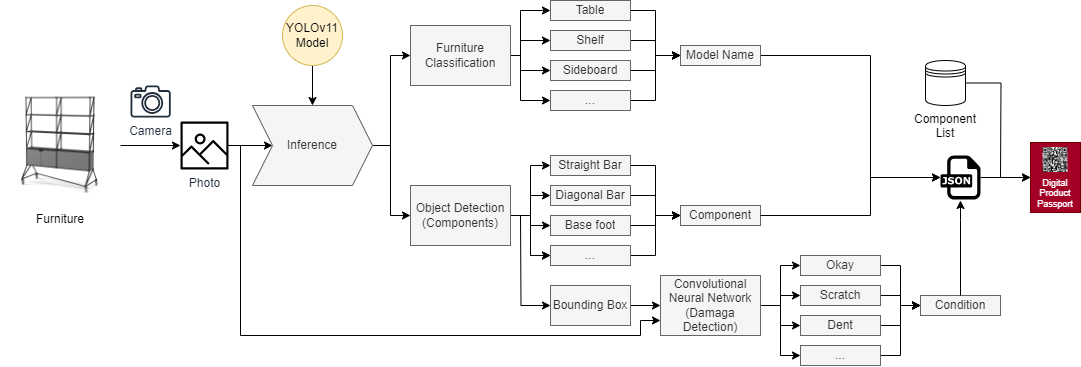
\includegraphics[width=1\linewidth]{images/architecture.png}
    \caption{High-level workflow from image capture to DPP generation.}
    \label{fig:concept}
\end{figure}

\paragraph{Data acquisition}
A user captures an image (or short video sequence) of a furniture object with a commodity camera.  The raw visual data serve as the single external input. No QR codes or RFID tags are attached to the components.

\paragraph{Visual inference}
The image is forwarded to an edge device -- an \emph{Nvidia Jetson Orin Nano} in our demonstrator -- where a YOLOv11 model performs two tasks in parallel:

\begin{itemize}
    \item \textbf{Furniture classification} predicts the overall product category (``Table'', ``Shelf'', \dots) and returns the catalogue \emph{model name}.  
    \item \textbf{Component detection} localises individual parts (``Straight Bar'', ``Diagonal Bar'', ``Base Foot'', \dots) and outputs bounding-box coordinates for each instance.
\end{itemize}

\paragraph{Damage detection}
For every detected bounding box a lightweight convolutional network performs \emph{damage detection}.  The network assigns a condition label such as \textit{Okay}, \textit{Scratch}, or \textit{Dent}.  These labels can later influence reuse or repair decisions.

\paragraph{Collection and graph storage}
The classified product, its component list, and the condition annotations are aggregated into a structured JSON document that adheres to a pre-defined template.  This document is ingested into a Neo4j graph database, where each physical part becomes a node and is linked to the \emph{Collection} node representing the furniture instance.  Because every part is always a member of exactly one Collection, the graph implicitly guarantees traceability without physical identifiers.

\paragraph{Digital Product Passport generation}
A mapper service converts the JSON graph fragment into a \emph{DPP} record. The resulting DPP bundles the detected component list, condition labels, and provenance links in a machine-readable form that can be exported, queried, or shared via a QR code or standard REST interface.

\paragraph{Training data}
To reach production performance, the visual models are trained on a hybrid dataset that combines manually labelled photographs with synthetically rendered images generated in NVIDIA Isaac-Sim.  Real images provide texture fidelity, while synthetic samples cover rare poses, occlusions, and lighting conditions that would be costly to capture manually.

\paragraph{Summary}
In summary, the concept replaces manual inventory and paper-based damage reports with an automated, camera-driven workflow.  By merging computer vision results with graph-based Collections, the approach fulfils the traceability requirements of the upcoming ESPR regulation while remaining free of physical IDs.

\subsection{Model Training}
\label{sec:model-training}

\paragraph{Datasets}
Two complementary datasets were used.  
First, a set of \emph{10\,000 synthetically rendered RGB images} was generated in NVIDIA Isaac-Sim and fully annotated with 2-D bounding boxes.  
Second, a markedly smaller set of \emph{approximately 1 000 real photographs} was captured in the factory and manually annotated.  
All annotations were produced and curated in Roboflow.  
Both datasets cover the same nine component classes -- \textit{Straight Bar, Diagonal Bar, Threaded Rod, Handle, Base Foot, System Shelf Panel, Front/Rear Panel, Side Panel, Double Door}.  
The synthetic set was split 80 \% / 20 \% into training (8 000 images) and validation (2 000 images); the real set followed the same ratio.

\paragraph{Detection models}
Three YOLOv11 variants were trained:


\begin{enumerate}
    \item \textbf{YOLOv11s (Custom)} -- trained on the real-photo subset to capture authentic lighting conditions and surface noise.
    \item \textbf{YOLOv11l (Synthetic)} -- trained exclusively on the 10\,000 synthetic Isaac-Sim images, providing broad viewpoint and occlusion coverage without relying on scarce real data.
    \item \textbf{YOLOv11s-seg (Nub detection)} -- trained with the segmentation head enabled to classify the up- and down-facing nubs captured by the left- and right-side cameras of the demonstrator.
\end{enumerate}


All models were trained with an input resolution of \(640\times640\) pixels, a batch size of 16, and 300 epochs using the default Ultralytics hyper-parameters (SGD optimiser, initial learning rate \(1\times10^{-3}\), weight decay \(5\times10^{-4}\)).  
Standard augmentations -- Mosaic, HSV shift, horizontal flip, and random scaling -- were enabled to improve robustness against changing perspectives and illumination.

\paragraph{Condition classifier}
For surface-damage assessment a pruned, half-precision VGG-16 was trained on cropped bounding-box patches.  
Each patch was labelled as \textit{Okay}, \textit{Scratch}, or \textit{Dent}.  
Data augmentation (random rotation and Gaussian noise) mitigated class imbalance in the real-world damage samples.

\paragraph{Performance}
The best configuration, obtained with the YOLOv11l model fine-tuned for 300 epochs, achieved a mean average precision of \(\mathrm{mAP}_{50}=0.75\) and \(\mathrm{mAP}_{50:95}=0.596\) on the held-out validation set.  
These figures are adequate for automated inventory and serve as the baseline for the downstream DPP workflow described in Section~\ref{sec:dpp-integration}.

\subsection{Information Extraction}
\label{sec:info-extraction}

Once the detection stage delivers class labels and bounding boxes for every visible component, a second processing layer derives additional attributes that are required by the DPP.

\paragraph{Geometric measurement}
Each image contains a printed \texttt{Aruco} marker placed on the inspection platform.  
Because the marker size is known, the pixel-to-millimetre ratio can be computed for every frame.  
The physical length of elongated components (e.g.\ \emph{Straight Bar}, \emph{Diagonal Bar}) is then estimated by multiplying the bounding‐box diagonal with this ratio.  
This automated procedure provides length data suitable for stock-keeping and matching against catalogue information.

\paragraph{Appearance features}
Colour and decor information influence both aesthetic decisions and reuse potential.  
For each detected part a colour histogram in the CIE\-Lab space is recorded and stored as a vector in the graph database.  
If required, a decor‐matching module compares this vector with a reference palette to assign finish labels such as \textit{Powder‐coated white} or \textit{Stainless steel}.  These labels are appended to the corresponding component node in Neo4j and become part of the exported DPP.

\paragraph{Condition and quality assessment}
Bounding-box crops are forwarded to a pruned, half-precision \emph{VGG-16} network.  
The model assigns one of the surface-condition labels (\textit{Okay}, \textit{Scratch}, \textit{Dent}, ...) to each component.  
The resulting label is written back to the corresponding component node in the Collection graph, enabling downstream decisions such as routing damaged parts to refurbishment or excluding them from reuse scenarios.

\paragraph{Vision-Language Model (VLM)}
An initial VLM prototype was implemented, where a local large language model (LLM) was combined with the object recognition results from the computer vision module to identify potentially unrecognised components.
The modular structure of the furniture components provides explicit spatial and semantic relationships that are particularly valuable for the VLM approach. For example, the arrangement of two intersecting straight bars can be used to derive constructions that are typically stabilised by connecting elements such as screws and nut rods.
The bounding boxes and their geometric properties (in particular coordinates and position) were transferred to the VLM. 
Then, based on these features, an analysis was performed to determine whether there were functional relationships between components that were not recognised by the original object recognition. Missing components that could be inferred from the context were then suggested to the user for confirmation (human in the loop).


\paragraph{Metadata integration}
The extracted geometric, appearance, and condition metadata are written back to the Collection graph and ultimately exported with the DPP, giving downstream users a machine-readable summary of each component’s physical properties and current state.

\subsection{Digital Product Passport Integration}
\label{sec:dpp-integration}

All recognition results are consolidated in a Neo4j graph database, which forms the permanent backbone of the DPP. The graph model distinguishes between three main node types: \texttt{Order}, \texttt{Image} and \texttt{Component}, which are linked to each other by the relationships \texttt{PART\_OF} and \texttt{BELONGS\_TO}. 
Each component node stores the attributes extracted in the previous processing stage regarding geometry, appearance and condition, together with a globally unique identifier that enables subsequent updates and cross-references. 
Location and contact metadata are additionally attached via special \texttt{Location} nodes. This information is used to calculate the resource efficiency and transport emissions saved by online detection of the status instead of on-site detection.

\paragraph{Graph persistence}
Whenever an operator confirms the automatically generated detections in the web interface, the validated data are written to Neo4j in a single Cypher transaction.  The query either merges existing nodes or creates new ones, ensuring that the graph stays consistent even under concurrent use.  By executing all write operations atomically, the system guarantees that component nodes are always linked to their corresponding image and order nodes.

\paragraph{Resource-efficiency analytics}
Two lightweight analytics routines run directly on the graph data.  The first aggregates reusable components to estimate material savings in terms of avoided steel mass and associated CO\(_2\) emissions.  The second derives transport emissions by combining stored geo-coordinates with point-to-point distances and mode-specific emission factors.  Both routines return structured results that are rendered in a dashboard, giving users an immediate overview of material utilisation and logistics impact at order level.

By unifying component attributes, spatial metadata, and sustainability metrics in a single property graph, the system realises a machine-readable DPP that can be queried in real time and incrementally enriched as new information becomes available.

\section{Results}
\label{sec:results}

\subsection{Physical Demonstrator}
\label{sec:results-demonstrator}

Figure~\ref{fig:demo-photo} shows the mobile inspection rig that was built to evaluate edge inference.  
The aluminium frame carries two side-mounted industrial cameras and a 4 K webcam in a top-down position, providing three complementary views of the component under test.  
All image streams are processed locally on an \emph{NVIDIA Jetson Orin Nano}, which executes the detection pipeline in real time.  
A monitor mounted above the frame provides immediate visual feedback to the operator. The signal flow and main processing steps of the demonstrator are summarised in the block diagram in Figure~\ref{fig:demo-block}.

\begin{figure}
    \centering
    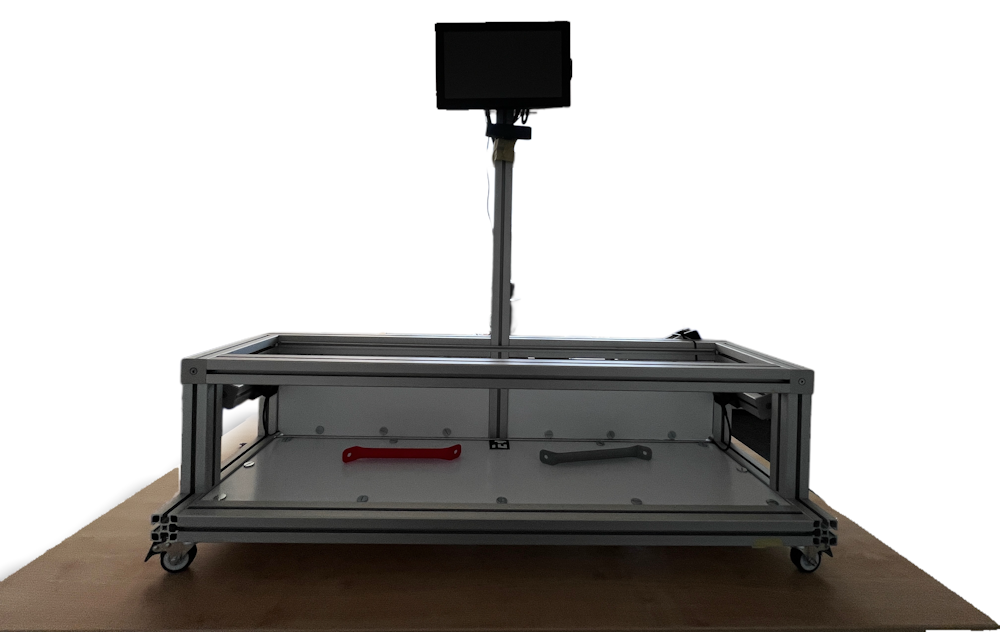
\includegraphics[width=0.65\linewidth]{images/demonstrator-assembled.png}
    \caption{Photograph of the mobile inspection demonstrator with three cameras and on-board monitor.}
    \label{fig:demo-photo}
\end{figure}

\begin{figure}
    \centering
    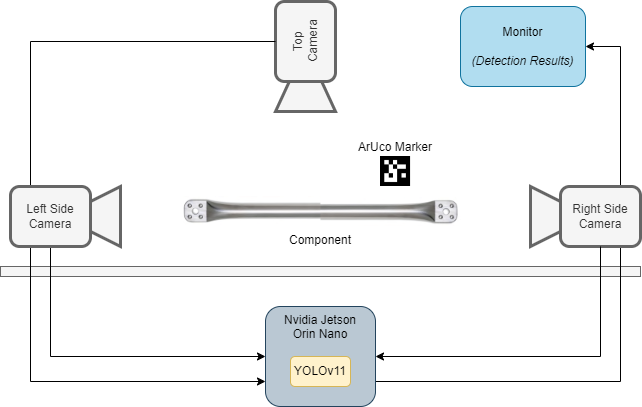
\includegraphics[width=0.65\linewidth]{images/demonstrator.png}
    \caption{Block diagram of the demonstrator: three cameras feed the Jetson Orin Nano, which runs YOLOv11 for object and defect detection and streams the results to the monitor.}
    \label{fig:demo-block}
\end{figure}


\paragraph{Run-time behaviour}
With FP16 inference and an input resolution of \(320\times320\) pixels, the system delivers smooth real-time feedback on the on-board monitor; increasing resolution to \(640\times640\) in full precision noticeably reduces frame rate but still remains within interactive bounds.  
This confirms that the network backbone and damage-detection head can operate entirely on low-power edge hardware, eliminating the need for a cloud connection during inspection.

\paragraph{Qualitative results}
The top camera -- running the combined YOLOv11s (real) and YOLOv11l (synthetic) ensemble -- reliably identifies the nine target component classes, while the side cameras run the nub-orientation segmentation model to determine up- or down-facing connectors.  
Detected parts are highlighted on the live display together with their condition label (\emph{Okay}, \emph{Scratch}, or \emph{Dent}).  
Shop-floor trials demonstrated that the visual overlay is sufficiently responsive for an operator to reposition parts in real time until a clean detection is achieved.

\paragraph{Practical implications}
The entire demonstrator is built from off-the-shelf components, fits on a standard workshop trolley, and runs on a single 230 V outlet.  
Because all processing takes place on the Jetson, the setup remains functional in network-constrained environments and can be duplicated at low cost.  
The qualitative evaluation shows that edge-based detection is a viable alternative to manual inspection for modular furniture components; rigorous quantitative benchmarking will be the focus of future work.

\subsection{Web Application}
\label{sec:results-webapp}

The web front-end provides a user-friendly interface for uploading images, reviewing detections, and persisting confirmed data to the DPP graph.

\paragraph{Technology stack}
The backend is implemented in \texttt{FastAPI} running on Python~3.10 and served by the \emph{Uvicorn} ASGI server.  
A lightweight Docker image (\texttt{python:3.10-slim}) bundles the application together with all model artefacts.  
The presentation layer uses Jinja templates styled with Bootstrap.

\paragraph{Core API endpoints}
The route \texttt{/detect/} accepts single or batched image uploads and returns raw detection results in JSON format.  
After manual review, the browser posts the amended data to \texttt{/confirm-results/}, which writes the final component, image, and order nodes to Neo4j.  
Additional endpoints handle colour-decor analysis (\texttt{/detect-decor/}) and live video streams, enabling both still-image and continuous-feed operation.

\paragraph{User-interface}
The result view (Fig.~\ref{fig:website}) overlays bounding boxes and class labels on the uploaded image and lists the detected component ID, confidence, condition state, and, where applicable, the inferred colour or coating together with HEX and NCS codes.  
Operators can adjust misclassified items, add optional order metadata, and commit the record to the graph by clicking \emph{Save to Neo4j}.  
All feedback is rendered server-side; the browser merely submits HTML forms, ensuring compatibility with low-spec devices.

\paragraph{Performance}
On a standard laptop the synchronous \texttt{/detect/} call returns in well under a second for medium-resolution images, dominated by the YOLOv11 inference time.  No end-to-end latency bottle-neck was observed during user tests. Although no standalone export endpoint is yet provided, the confirmed detections written to Neo4j constitute the authoritative source for the DPP described in Section~\ref{sec:dpp-integration}.

\paragraph{Source code}
The complete web application, including Docker recipes and configuration files, is available under an open licence at: \url{https://github.com/Green-AI-Hub-Mittelstand/SUSPEKT}.

\begin{figure}
    \centering
    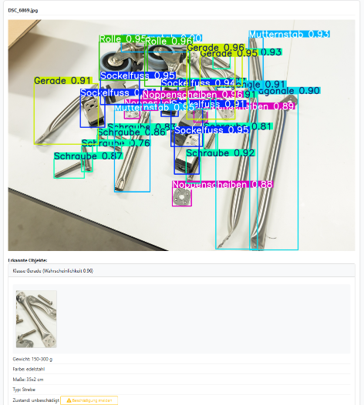
\includegraphics[width=0.45\linewidth]{images/system180_ism.png}
    \caption{Screenshot of the web interface showing detected components with class labels and confidence values.}
    \label{fig:website}
\end{figure}

\section{Discussion}
\label{sec:discussion}

The results demonstrate that computer-vision pipelines can now generate the core data required for a DPP without relying on physically attached identifiers such as QR codes or RFID tags.  By assigning every detected component to a Collection node in Neo4j, the system achieves continuous traceability even when parts are disassembled and reused -- an essential capability for modular furniture that is re-configured many times during its service life.

The study confirms that modern object-detection and colour-classification networks can extract geometry, condition, and décor information directly from images and video streams.  Such “AI-generated attributes” align well with the European Commission’s call for AI-based services that populate DPPs, reducing manual data entry and improving data freshness.

Training the YOLOv11l model exclusively on 10 000 synthetic images delivered a \(\mathrm{mAP}_{50}=0.75\) despite the limited real-photo corpus.  This underlines the practical benefit of simulation-generated data for rapid model boot-strapping and incremental expansion as new components appear.

First experiments with a Vision-Language Model suggest that topological relations -- such as \emph{“Diagonal Bar connected between two Straight Bars”} -- can be inferred from paired images and text prompts.  Such relational cues could fill blind spots when parts are occluded or entirely absent from a photo, further reducing the need for manual confirmation.

Although the present work stores all information in Neo4j, long-term interoperability will require mapping the Collection graph to agreed-upon ontologies and vocabularies.  Standards such as IEC 63278-1 (Asset Administration Shell, AAS) and the modular \emph{Ontology Design Pattern} (ODP) approach for DPPs~\cite{Pourjafarian2025} provide reusable building blocks that avoid monolithic schemas while ensuring semantic alignment.  Integrating these patterns with the AAS meta-model can further promote cross-domain data exchange.

The current prototype lacks fine-grained user rights, and the length-estimation routine has yet to be benchmarked rigorously.  Future work will integrate incremental on-device learning to accommodate new parts, extend the Web UI with drag-and-drop collection transfer, and include a formal DPP export compliant with upcoming ESPR guidelines.

\section{Conclusion and Outlook}
\label{sec:conclusion}

This study demonstrates that a camera-based, ID-free workflow can generate the core data required for a DPP in the domain of modular furniture.  By combining YOLOv11 object detection, color and condition analysis, and a graph-based Collection model, the system achieves end-to-end traceability without QR codes or RFID tags.  Synthetic images proved sufficient to bootstrap accurate detection models, while a Neo4j property graph provides a flexible substrate for life-cycle analytics such as material-savings and transport-emission estimates.

The concept scales naturally to new product variants, because additional components can be introduced through incremental training and do not require hardware changes.  Nonetheless, several limitations remain: (i) length measurements are based on single Aruco markers and warrant a systematic accuracy study; (ii) disassembly scenarios have not yet been validated in industrial settings; (iii) the current prototype lacks fine-grained user-rights management and a formal ESPR-compliant DPP export.

Future work will address these gaps by integrating multi-marker photogrammetry for improved geometry capture, extending the Web UI with drag-and-drop collection transfer to support disassembly workflows, and mapping the Neo4j schema onto standard AAS or ODP vocabularies.  We also plan to evaluate on additional material classes and embed on-device incremental learning to keep the models current without full retraining.  With these enhancements, the approach presented here can serve as a practical blueprint for AI-assisted, circular-economy data pipelines in other modular product domains.

\bibliography{references}
\bibliographystyle{elsarticle-harv}

\end{document}

